\documentclass[pdf,bookmarks,colorlinks=true]{IEEEtran}
\usepackage{times}
\usepackage{amsmath}
\usepackage{hyperref}
\usepackage{url}
\usepackage{psfrag}    %Shouldn't use this if you plan on using pdflatex!
\usepackage{graphicx}
\usepackage{wrapfig}   %for wrapping text around figures and tables

%Included for Gather Purpose in WinEdt only:
%input "rc.bib"

\title{\bf Know vulnerabilies OSS libraries}

\author{Ronaldo Canesqui\\
Southern Adventist University\\
ronaldocanesqui@southern.edu
}
\graphicspath{{Images/}}
\begin{document}

\maketitle

\begin{abstract}

The abstract should describe the basic message of the paper, including: the
problem, why your solution should be of interest, some notion that your
solution is effective, and a teaser about how it has been evaluated. Cover all
of this using between 75 and 150 words. The abstract is thus the hardest part
to write. Sometimes I try to write it first, but the final version is usually
composed of items drawn from the introduction, and then condensed, as the last
step of writing the paper.

\end{abstract}

%   \tableofcontents
%   \newpage

% \doublespace

\section{Introduction}
\label{sec:Introduction}

\textbf{The problem we have solved:}

%\begin{itemize}
%\item
The use of open-source libraries is a factual reality in the software industry. In 2018, Synopsys\footnote{https://www.blackducksoftware.com/} found open-source code in more than 96\% of their audits\cite{Synopsys2019}. OSS \footnote{Open-Source Software} usage has increased exponentially during the last decade. The most popular source for libraries in the Java ecosystem, Maven Central Repository, growth 542.17\% from 2010 to 2016 \cite{Kula2018}. Another popular open-source repository for the Javascript ecosystem, npm growth from 0 packages at its creation in 2010 to 1,000,000 packages in 2019. \footnote{https://snyk.io/blog/npm-passes-the-1-millionth-package-milestone-what-can-we-learn/ accessed 10/10/2019}  
The figure~\ref{PackageEvolution}\cite{Decan} shows the number of packages evolution on other popular ecosystems.
\begin{figure}[h]
	\centering
	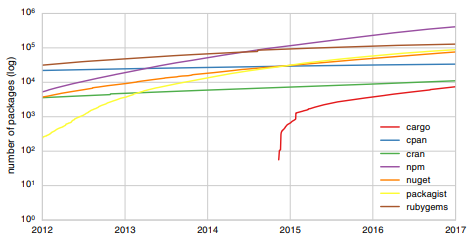
\includegraphics[scale=0.70]{PackagesEvolution.png}
	\caption{Evolution of the number of packages.}
	\label{PackageEvolution}
\end{figure}
%\item
How to leverage the power of open source libraries and still manage the risk of vulnerabilities they carry is a problem that either remain ignored by many software engineers or present considerable challenges to them.

%\end{itemize}


\textbf{Why the problem is not already solved or other solutions
are ineffective in one or more important ways}

A 2014 study from Sonatype determined that over 6\% of the download requests from the Maven Central Repository were for component versions that included known vulnerabilities. In their review of over 1,500 applications, each of them had an average of 24 severe or critical flaws inherited from their components. \footnote{Report published January 02, 2015 at http://goo.gl/i8J1Zq.}
A white paper produced by Contrast security, stated that over 25\% of all libraries download from Maven Central Repository has vulnerability. Only one vulnerable version of the Java GWT package was downloaded 17,666,703 times \cite{williams2012unfortunate}.
Among the 10 most popular npm packages, 6 present 1 or more vulnerabilities \footnote{(https://snyk.io/blog/npm-passes-the-1-millionth-package-milestone-what-can-we-learn/ accessed 10/10/2019)}.

In a study on security vulnerabilities impact\cite{Decan2018} the researchers found that out of 610,097 available packages (2017 data) 133,602 packages directly depend on a vulnerable package and 72,470 packages had at least one release that relies on a vulnerable package.
In the same study, they also found a crescent number or vulnerabilities in the npm repository. The figure~\ref{SVEvolution} shows he evolution of the number of vulnerabilities and the impact on dependent packages. Comparing 2014 data, where the distinct packages (doted lines) impact almost the same number of dependent package (straight lines), with 2017 data, it is evident the  tendency of increasing impact on dependent packages.

\begin{figure}[h]
	\centering
	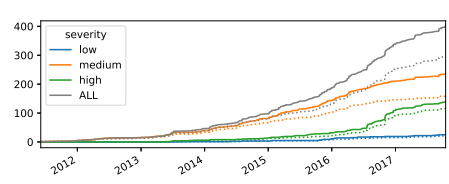
\includegraphics[scale=0.70]{SVEvolution.png}
	\caption{Evolution of the number of discovered vulnerabilities (straight lines) and corresponding distinct packages (doted lines) per severity.}
	\label{SVEvolution}
\end{figure}

%\end{itemize}


\textbf{Why our solution is worth considering and why is it effective
in some way that others are not}

%\begin{itemize}
%\item
During this paper studies related to dependencies management will be presented along with the most recent studies about how to identify know vulnerabilities in open source libraries.
%\item
The rest of this paper will cover studies on how long vulnerable package remains harmful and how long a fix takes to spread over the dependent applications \ref{sec:VulnerabilityTimeFrame}, what prevents software developers from updating their dependencies (section III) and solutions on how to manage the risk involved on open source libraries adoption.  
 %\item
The rest of this paper first discusses related work in
\ref{sec:RelatedWork}, and then describes our implementation in
\ref{sec:Implementation}. \ref{sec:Evaluation} describes how we evaluated
our system and presents the results. \ref{sec:Conclusion} presents our
conclusions and describes future work.
%\end{itemize}
\section{Vulnerability Timeframe}
\label{sec:VulnerabilityTimeFrame}


%\begin{itemize}
%\item
To analyze for how long a vulnerability is harmful the study \cite{Decan2018} used a 700 security vulnerabilities report made available by Snyk.io \footnote{https://snyk.io} and retrieved the list of its releases from the open source discovery service libraries.io \cite{Nesbitt2017}. Based on the list of releases, they identified which ones were affected by the vulnerability.
Based on the relationship between package, vulnerability, first release data, vulnerability discovery date, it was possible to trace a vulnerability timeframe.

\textbf{How long does the package remains vulnerable}
%\item
Figure~\ref{RemainsVulnerable} shows Kaplan-Meier estimator  curve \cite{Kaplan1958} for the event “vulnerability is fixed”. The data presented considers the date of the affected release and the date that the fix was available. After 10 months, there is a probability higher than 80\% that a high severity vulnerability is still unfixed.

\begin{figure}[h]
	\centering
	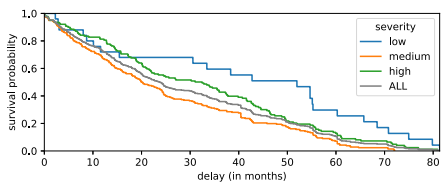
\includegraphics[scale=0.70]{RemainsVulnerable.png}
	\caption{Survival probability for event “vulnerability is fixed” w.r.t. the date of first affected release.}
	\label{RemainsVulnerable}
\end{figure}

%\end{itemize}


\textbf{When a vulnerability is discovered}
%\item 
Figure~\ref{WhenDiscovered} shows that most severities are discovered in old packages. 75\% of all vulnerabilities are found in libraries older than 13 months. Even tough it was not highlighted in the original study, the shorter wave in high severity vulnerabilities may suggest the higher priority in which they are handled, especially when compared to the low severity graph that shows smother curves. Most severities are found in packages older than 28 months.

\begin{figure}[h]
	\centering
	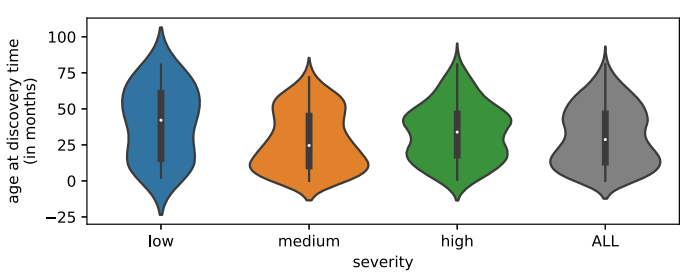
\includegraphics[scale=0.45]{WhenDiscovered.png}
	\caption{Violin plots of packages age at discovery time by vulnerability severity.}
	\label{WhenDiscovered}
\end{figure}

%\end{itemize}

\textbf{When a vulnerability is fixed}
%\item 
Most of the vulnerabilities are fixed between the discovery date and the public announcement. Figure~\ref{WhenIsFixed} shows that there is a probability of 50\% of a fix becomes available in the first month after discovery. And 80\% of all vulnerabilities are fixed between 12 and 13 months. After 20 months of the discovery all high severity vulnerabilities were fixed. Some medium severity vulnerabilities, according to the graph, will take more than 40 months to be fixed.

\begin{figure}[h]
	\centering
	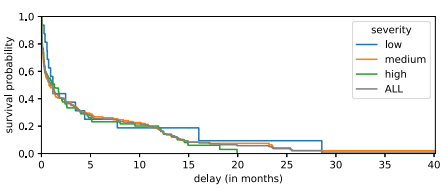
\includegraphics[scale=0.75]{WhenIsFixed.png}
	\caption{Survival probability for event "vulnerability is fixes" w.r.t. vulnerability discovery time.}
	\label{WhenIsFixed}
\end{figure}

%\end{itemize}


\textbf{When a vulnerability is fixed in a dependent package}
%\item 
The impact on dependent packages is important due to increasing number of dependencies, faster then the number of available packages. The figure~\ref{DependenciesGrowing} shows a more step curve when compared to the number of available packages (figure~\ref{PackageEvolution}). 
Figure~\ref{WhenIsFixedDependentPackages} shows that after 20 months, 100\% of  high severity vulnerabilities are fixed while there are 40\% of the dependencies vulnerable at the same time. The slowness on updating dependencies found in this study is supported by similar findings in different studies covering a wide range of ecosystems such as SmallTalk\cite{Robbes:2012:DRA:2393596.2393662}, Pharo\cite{7332471}, Java \cite{7816485}, Apache products\cite{Bavota2015}, Windows ecosystem \cite{7163055}, and Javascript ecosystem \cite{Lauinger}.

\begin{figure}[h]
	\centering
	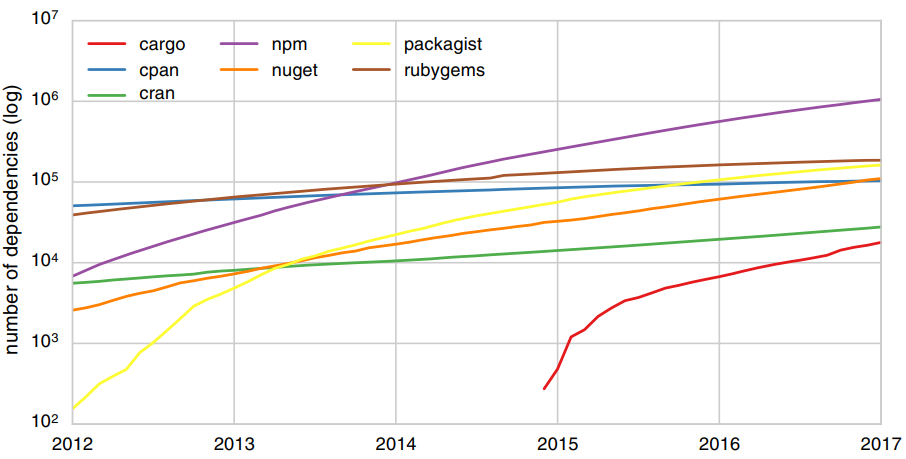
\includegraphics[scale=0.40]{DependenciesGrowing.png}
	\caption{Evolution of the number of dependencies (considering for each point in time the latest available
		release of each package).}
	\label{DependenciesGrowing}
\end{figure}

\begin{figure}[h]
	\centering
	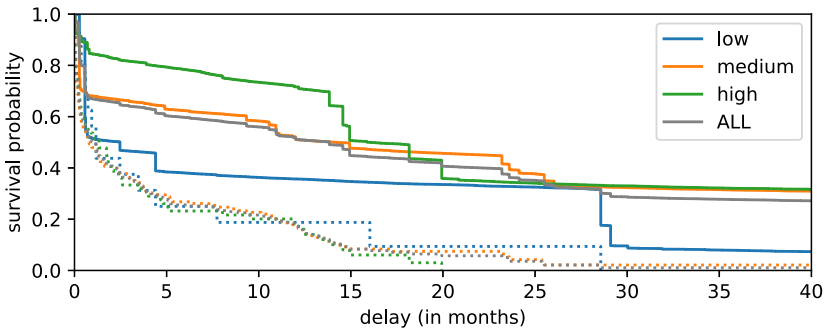
\includegraphics[scale=0.40]{WhenIsFixedDependentPackages.png}
	\caption{Survival probability for event “package is fixed” w.r.t. vulnerability discovery time. Dependent packages are
		shown as straight lines and upstream packages as dotted lines.}
	\label{WhenIsFixedDependentPackages}
\end{figure}

%\end{itemize}

\section{Developer's Timeframe}
\label{sec:DevelopersTimeFrame}


%\begin{itemize}
%\item
To understand the vulnerabilities timeframe it is required to understand the application's maintainer behavior on updating and selecting their dependencies. A study \cite{Derr2017} conducted with 203 app developers from Google Play clarified the following research questions: What is the common workflow to search for and to integrate third-party libraries into applications? How frequently do developers update their apps/libs and what is their main motivation for updates?
What are possible reasons to not update dependencies and what solutions could app developers think of?
%\item 
Based on the applications maintainer's answers, the study conclude that 78\% of them do not have a fixed schedule for app update (Figure~\ref{IsYourAppUpdatedFixedSchedule}) and only 33\% of them mention a library update as a reason to update their app (Figure~\ref{ForWhichReasonUpdate}). When the maintainers were questioned why do you update your app's libraries, 96.47\% of them answered bug fixing and 57.65\% mentioned security (figure~\ref{WhyDoYouUpdateYourLibrary}). Regarding library selection criteria, only 26.58\% answered security, even thought the answer update frequency is related and received 35.16\% of the votes (figure~\ref{LibrarySelectionCriteria}). When asked reasons why your app would include outdated libraries?, 57.03\% answered that the library was still working, 50\% answered to prevent incompatibilities and 32.81\% were unaware of updates (figure~\ref{ReasonsOutdatedLibrary}).

\begin{figure}[h]
	\centering
	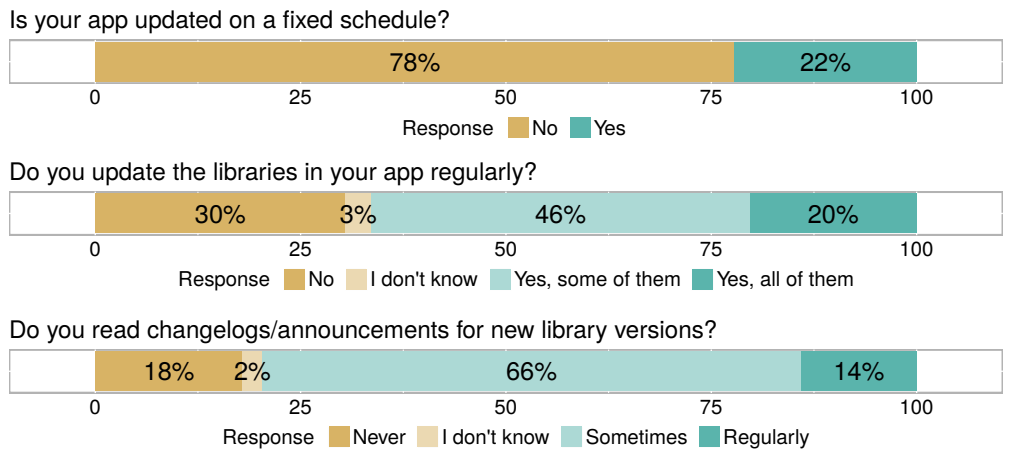
\includegraphics[scale=0.30]{IsYourAppUpdatedFixedSchedule.png}
	\caption{Anwsers for questions regarding app/library release frequency.}
	\label{IsYourAppUpdatedFixedSchedule}
\end{figure}
\begin{figure}[h]
	\centering
	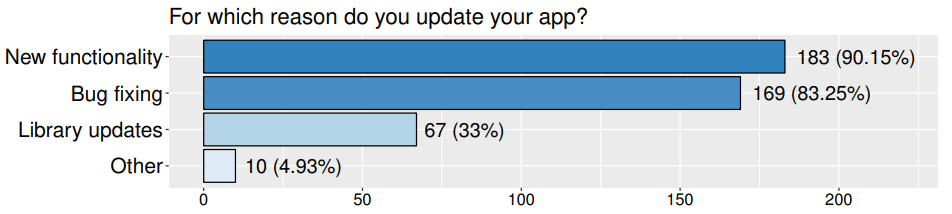
\includegraphics[scale=0.35]{ForWhichReasonUpdate.png}
	\caption{Answers for questions:For which reason do you update your app?}
	\label{ForWhichReasonUpdate}
\end{figure}
\begin{figure}[h]
	\centering
	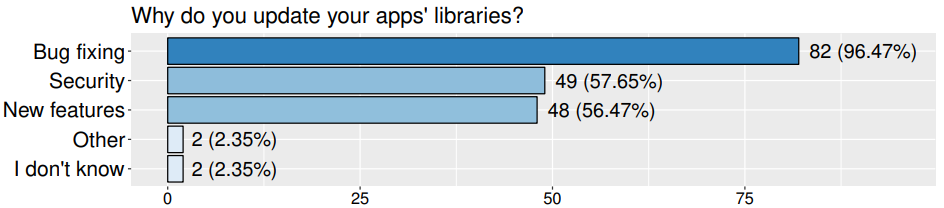
\includegraphics[scale=0.35]{WhyDoYouUpdateYourLibrary.png}
	\caption{Answers for questions: Why do you update your apps' libraries?}
	\label{WhyDoYouUpdateYourLibrary}
\end{figure}
\begin{figure}[h]
	\centering
	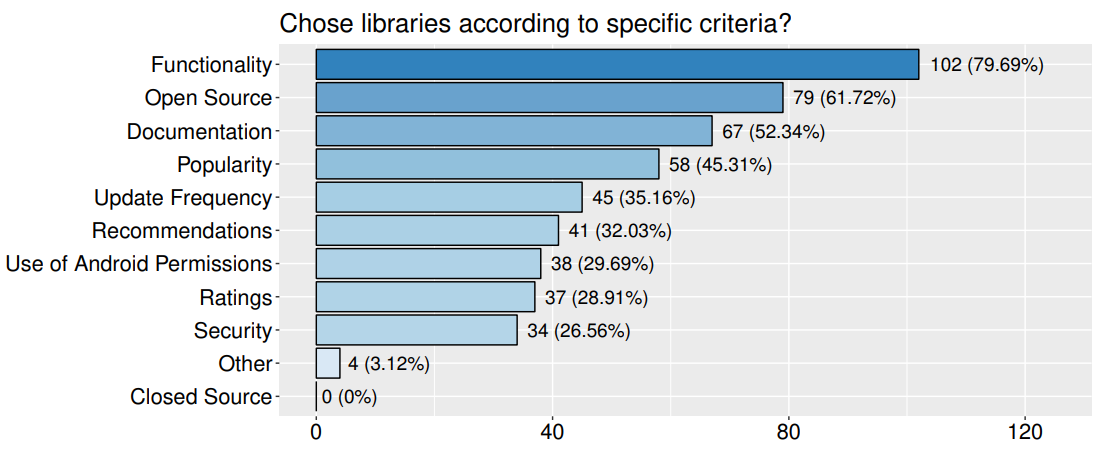
\includegraphics[scale=0.30]{LibrarySelectionCriteria.png}
	\caption{Answers for questions: Chose libraries according to specific criteria?}
	\label{LibrarySelectionCriteria}
\end{figure}
\begin{figure}[h]
	\centering
	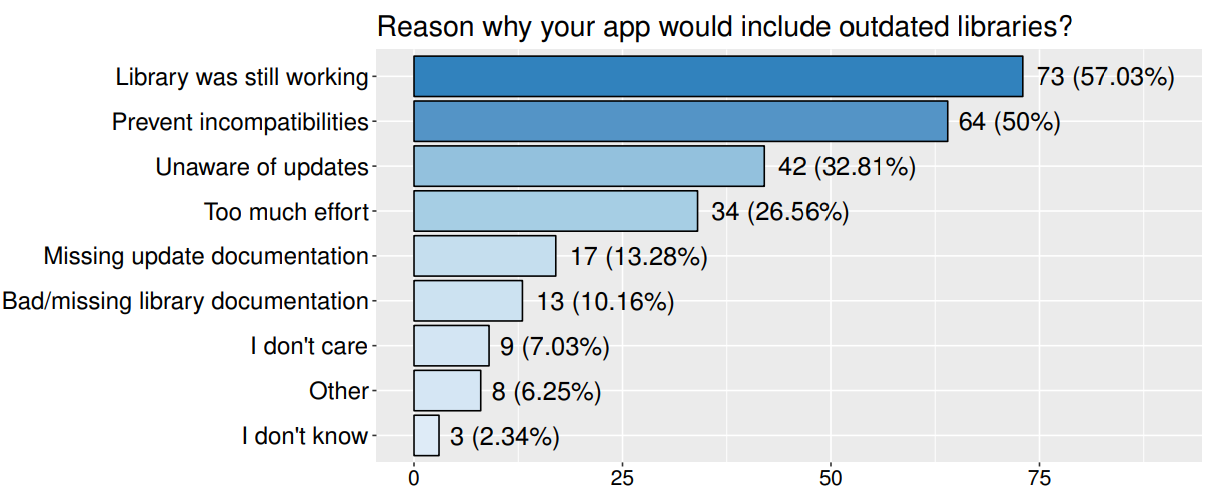
\includegraphics[scale=0.28]{ReasonsOutdatedLibrary.png}
	\caption{Answers for questions: Reason why your app would include outdated libraries?}
	\label{ReasonsOutdatedLibrary}
\end{figure}

%\begin{itemize}
%\item 
The study concludes that the main reasons to keep a library outdated are incompatibility prevention, unaware of updates and too much effort. Other study on this field \cite{Kula2018} reaches at the same conclusion regarding why maintainers keep outdated dependencies. On following sections, studies that proposed ways to deal with those main problems are presented along with their conclusions.

%\end{itemize}
\section{Increasing awareness and reducing effort on dependency management}
\label{sec:IncreasingAwarenessReducingEffort}

%\begin{itemize}
%\item
Various researchers have worked to solve the problem of know vulnerabilities in open source packages and their dependencies. In this section, the most recent works will be presented along with their conclusions.

\textbf{Predicting vulnerabilities:}
%\begin{itemize}
%\item
Even thought the focus of this work is on papers that detect vulnerabilities using know vulnerabilities database, it is worth mentioning that there is a branch of proposed solutions that operates identifying vulnerabilities based on a set of characteristics. Part of this solutions uses machine learning to identify vulnerabilities. One of this works \cite{Perl2015} mapped the CVE entries to the commit that generated the vulnerability and trained a SVM-based model using the commit's metadata. According to the authors this method reduced the amount of false positives by 99\% when compared to Flawfinder\footnote{https://https://dwheeler.com/flawfinder/}. It was capable of detecting 53 of the 219 known vulnerabilities used in the study and only producing 36 false positives. The proposed solution analyses each commit and tries to predict the presence of vulnerabilities.
%\end{itemize}

\textbf{Measuring dependency freshness}
%\begin{itemize}
%\item
The study \cite{Cox2015} proposes a method to measure the dependency freshness. The authors used information from project's pom.xml file to determiner what is the version being used and used the Maven Central Repository to determine the release history for the library. Based on this information, the authors were able to classify each used component in a risk profile with 4 categories: low, moderate, high and very high.
To determine the relationship between their risk profile and the security vulnerabilities the researchers matched the dependencies list and tried to match with the CVE vulnerability database. They were able to find a correlation between their freshness index and the number of vulnerabilities. The median variance of the rating, the researchers were able to classify the systems according to dependency freshness:
\begin{itemize}
	\item \textbf{Stable} Systems with a stable dependency freshness rating. The system dependencies see little to no updates.
	\item \textbf{Improving} Systems with an increasing dependency freshness
	rating. Dependencies are updated faster than they are released.
	\item \textbf{Declining} Systems with an decreasing dependency freshness
	rating. Dependencies are updated slower than they are released.
\end{itemize}

The metrics presented have a great potential in quantifying the dependency freshness. The method has at least one serious limitation: only direct dependencies can be measure, which can generate wrong classifications, specially when direct dependency is updated but a transient dependency exists and is outdated.  

\textbf{Library updatability}
%\begin{itemize}
%\item
The study \cite{Cox2015} was able to correlated library freshness with number of vulnerabilities. The finding that old libraries carry more vulnerabilities is also supported by other works \cite{Decan2018,Synopsys2019}. The study \cite{Derr2017} proposes an automated method to evaluate the updatability of dependencies. Their method consist of three steps: determine the API robustness, determine the library usage and determine the library updatability.
%\item
To determine the API robustness, the researchers extracted the public API from multiple versions of the same library, resulting in a library version/API pair list. According to authors this is a more fine-grained approach compared to \cite{Backes2016}. The authors then proceed with the library usage, where they inspect the bytecode looking for call to the API. Finally they matched the library version/APi pair list with the library usage to produce the library updatability, which informs what is the latest version the API can be updated to without causing incompatibilities.

The authors test their approach analyzing 98 libraries and 1,246,118 apps from Google Play. The results shows that in 85.6\% of the cases the identified library can be upgraded by at least one version (Upgrade1+) and on 48.2\% of the cases the library can be updated to the most current version simply by replace the old library, without any code change. Figure~\ref{LibraryUpdatability} shows the library updatability from their study.
 
\begin{figure}[h]
	\centering
	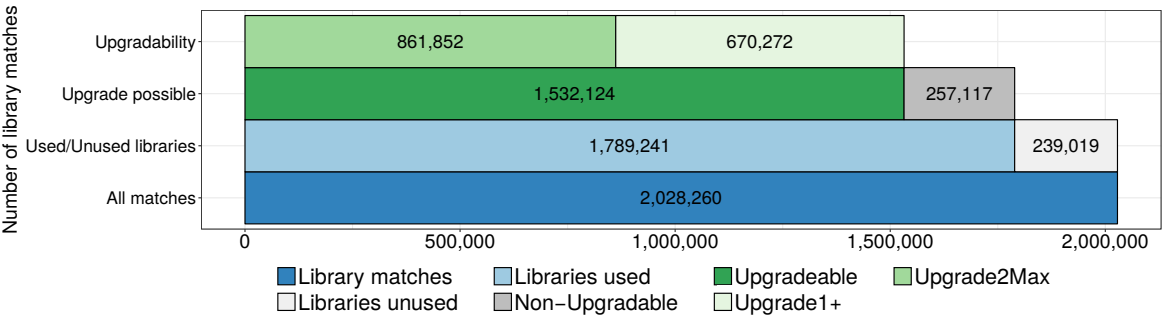
\includegraphics[scale=0.28]{LibraryUpdatability.png}
	\caption{Library updatability of current apps on Google Play.}
	\label{LibraryUpdatability}
\end{figure}


%\end{itemize}

\textbf{Vulnerability Alert Service (VAS)}
%\begin{itemize}
%\item
The Vulnerability Alert Service (VAS) is proposed by \cite{Cadariu2015}. Their focus is to increase the awareness about known vulnerabilities by making it part of the software quality process. The overall process is illustrated by figure ~\ref{VASProcess}. The target project has its dependencies extracted and recognized. The list of dependencies is then analyzed by the matching task, which tries to match the dependency with a entry from the vulnerability disclosures, in this study a CVE entry. Upon a successful match, an alert is produced which is consumed by a human operator. The authors extended the OWASP Dependency Check Tool to extract the dependency list from Maven pom.xml files and used this tool as the vulnerability checker described in the diagram.
%\item
The conclusion of this work shows a false positive rate of over 70\%, but the authors state that the rate is smaller when the solution was actually deployed. 
The researchers affirm that the high false-positive can be caused by situations like the MySQL-connector jar which is flagged with the vulnerabilities of the MySQL database server. The evaluation with the human operators shown that despite the false positive rate, an alert system was considered useful. Even the authors were satisfied with the operators' evaluation, since their solution looks for dependencies in pom.xml files, only direct dependencies can be identified.

\begin{figure}[h]
	\centering
	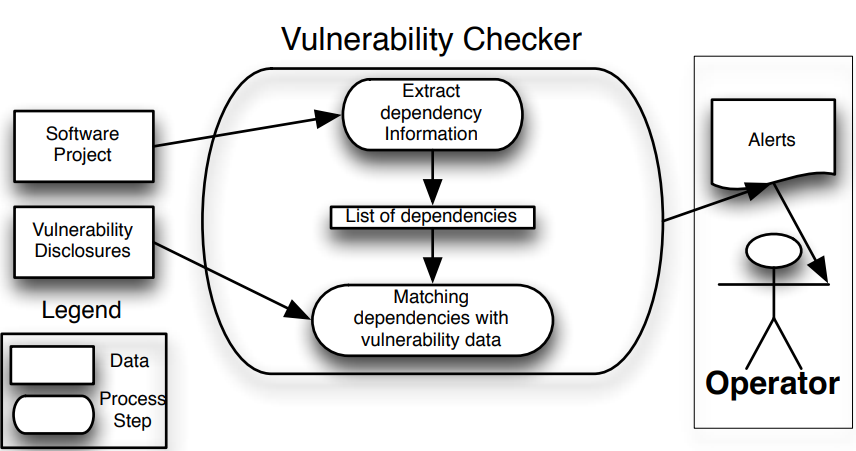
\includegraphics[scale=0.28]{VASProcess.png}
	\caption{The Vulnerability Alert Service process}
	\label{VASProcess}
\end{figure}
%\end{itemize}


\textbf{Code-based vulnerability identification}
%\begin{itemize}
%\item
The study \cite{Ponta2018} uses a method to identify vulnerabilities that, according to the authors, is more accurate then the methods proposed so far. Their work aims to answer the questions: does my application is vulnerable if it uses a vulnerable dependency? The researchers claim that this is not always the case and other studies failed to answer this question. The authors state that the software that contains a certain library that has known vulnerability does not need to be subject to costly efforts if proven that the vulnerability does not present harm. This way, the fix can be applied in the subsequent releases under no additional cost. Conceptually their solution can be used on any ecosystem, but their implementation is based on the Java ecosystem and the Maven Central Repository. They used the project’s pom.xml file to determine the dependencies. After the dependencies are determined, they remove all dependencies classified as provided and test, since those will not be deployed. Then the halted libraries are identified. 
One key aspect for this approach to work is a database vulnerability that contains the meta-data about library, such as name and version according to Maven Central Repository, the vulnerable source code and the source code for the fix. Using this database is possible to associate the dependency identified previously and the vulnerability, along with the source-code. This database was manually produced by the authors it covers 90\% of Java ecosystem vulnerabilities.
The authors used static analysis to determine if the vulnerable code is reachable and dynamically analysis. The dynamically analysis is done by instrumenting the vulnerable code and running automated and manual tests.
Their solution will notify the user if the vulnerability has impact on the application, meaning, the vulnerable code can be reached.
%\end{itemize}

%\item
Then, describe the structure of the rest of this section, and what each
subsection describes.
%\end{itemize}

\textbf{How our solution (will $|$ does) work}
%\begin{itemize}
%\item
This is the body of the subordinate paper describing your solution. It
may be divided into several subsections as required by the nature of your
implementation.

%\item
The level of detail about how the solution works is determined by what
is appropriate to the type of paper (conference, journal, technical report)

%\item
This section can be fairly short for conference papers, fairly long for
journal papers, or {\em quite} long in technical reports. It all depends on the
purpose of the paper and the target audience

%\item
Proposals are necessarily a good deal more vague in this section since
you have to convince someone you know enough to have a good chance of building
a solution, but that you have not {\em already} done so.

%\end{itemize}


\section{Evaluation}
\label{sec:Evaluation}

\textbf{How we tested our solution}
\begin{itemize}
\item   Performance metrics
\item   Performance parameters
\item   Experimental design
\end{itemize}


\textbf{How our solution performed, how its performance compared to
that of other solutions mentioned in related work, and how these results show
that our solution is effective}:

\begin{itemize}
\item   Presentation and Interpretation
\item   Why, how, and to what degree our solution is better
\item   Why the reader should be impressed with our solution
\item   Comments

\end{itemize}


\textbf{Context and limitations of our solution as required for
summation:} State what the results {\em do} and {\em do not} say.



\section{Conclusions and Future Work}
\label{sec:Conclusion}

\textbf{The problem we have solved}: The most succinct statement of the problem in the paper. Ideally one
sentence. More realistically two or three. Remember that you simply state it
without argument. If you have written a good paper you are simply reminding the
reader of what they now believe and of how much they agree with you.



\textbf{Our solution to the problem}: again, a succinct statement of the presented solution
Sometimes it works well to leave it at that and not even describe your
solution here. If you do, then again state your solution in one or two
sentences taking the rhetorical stance that this is all obvious. If you have a
good solution and have written an effective paper, then the reader already
agrees with you.

\textbf{Why our solution is worthwhile in some significant way}:
Again, a succinct restatement in just a few sentences of why your solution is
worthwhile assuming the reader already agrees with you

\textbf{Why the reader should be impressed and/or pleased to have read the paper}:
A few sentences about why your solution is valuable, and thus why the
reader should be glad to have read the paper and why they should be glad you
did this work.



\textbf{What we will (or could) do next}

\begin{itemize}
\item   Improve our solution
\item   Apply our solution to harder or more realistic versions of this problem
\item   Apply our solution or a related solution to a related problem

\end{itemize}


\bibliographystyle{IEEETrans}
\bibliography{./rc}


\end{document}
